\chapter{Evaluation \& Experiments}\label{sec:userTrials} % 6 pages
    
    In this chapter, we are going to discuss the user trials that were conducted at the end of the experiment and the results that were taken from these.

    \section{User Trials}
        Originally we were going to do user testing in person with the prospective users. This was to ensure that no problems would be encountered and that we could explain the steps in person before they started the testing. This was not possible as the project was not completely ready to be tested before the college shut down because of COVID-19. Instead, we created a suite of questions to ask users after they had completed using the recommender. In \ref{sec:UserTrialQuestions} we will explain the questions and the reasons behind them. As explained in section \ref{chap03-sec:3UserInteractionDesign} we designed a page to manage the use of the user trials so they can be conducted by the user by themselves. 

        Now that we were doing the user testing online we started with a small group of initial testers. This was used to iron out any bugs and to see if the questions were appropriate. When the application was set up for the user to begin testing we identified a few bugs. One of them was when explanations were being created there was a bug where the server would time out as they took too long to generate for one round. This was related to the number of movies in one's account and was fixed by changing the web server used. One type of explanation when created was using corrupt data. The API returned a not applicable string and this was entered into the database and used to create an explanation. This data was removed from the system to solve the error. Following this, we asked a number of people to use the system over the six rounds and to answer some questions at the end.

    
        \subsection{User Trial Questions}\label{sec:UserTrialQuestions}
        
            \begin{enumerate}
                \item In round 1 and 4 there were no titles or posters did this affect your choosing of a movie? if yes how important on a scale of 1-5 would you say posters and titles are?
                \item Did you notice anything different about the explanations in round 3 and 6 compared to other rounds?
                \item rounds 1,2,3 and rounds 4,5,6 had different movies. Did you notice a difference? was there a set that was better?
                \item On a scale of 1-5 would you find a system like this helpful?
                \item On a scale of 1-5 did you find this more interesting than a normal recommender?
                \item did you see any explanation types that were particularly interesting?
            \end{enumerate}

            We created these questions to evaluate the system that we had created. We wanted to find out what people thought about the system and whether it was a worthwhile use of their time. In question one we were referring to rounds one and four which were the first rounds using the different sets of movies. In these rounds, we did not show the user the movie titles or posters. They were only given the explanations we created. This was a test to see if the explanations we created contributed to a user picking a movie or if they were going to base it on the title and poster. We are hoping to see that most users found an explanation they liked and it was not just the best poster.
            In question two we asked whether users noticed a difference in rounds three and six. In these rounds, we changed the scoring system for the explanations to use random scoring where each explanation is given a random score. This was to test if people found explanations score with our scoring system more useful than random. There is a possibility that random will give some good results sometimes. 

            In question three we are asking the user if they noticed anything different about the sets of movies in the first three rounds vs the last rounds. The first three rounds take movies from the local cinema which should mean the user is  less likely to like the first set. The second set of movies were based on what a user's neighbours have rated highly. The original aim of the project was to use movies from the local cinema in the system. We wanted another set of movies to include so we used ones recommended by a user's neighbours.

            Question four and five were asked to see if the user found the system helpful or more interesting than a normal recommender they had used before. Hopefully, we will see that users have found the system helpful or even an interesting way of getting movie recommendations. 
            The final question was asked to see if any of the explanations in particular resonated with a user. This will probably be highly dependent on the person's tastes. The questions were sent out with some instructions on how to use the system to a group of people. 
         
        
       \subsection{Responses}

            
            \subsubsection{Question 1}
                we can see from the results of question 1 people think the movie poster and title are important in choosing a movie.This seems like an obvious conclusion since movies are inherently a visual medium. When someone is looking at a movie poster they get information about the movies such as the genre or style of the cinematography. They may also be able to recognise any actors that are in the movie. Neustar on behalf of Facebook evaluated 70 major studios across a variety of genres. These studios spent more than 1.8 billion on marketing in 2016. Over 80\% of this was on TV advertising. For example Avengers Endgame which was released in 2019 its budget was 356 million dollars. Another 200 million was spent just to advertise the movie. This movie grossed 2.8 billion dollars by the time it was finished showing around the world so money well spent. People seemed to regard the poster important. Although a few responses indicated that a neighbor's rating mattered more than the poster and title. As we can see from the results from question 1 in \ref{fig:Question1Results} people feel the poster and title are important.


                \begin{figure}
                    \centering
                    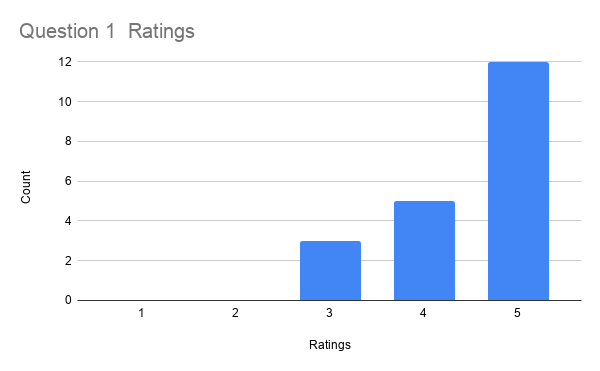
\includegraphics[width=100mm]{Question1Results.png}
                    \caption{Results from Question 1}
                    \label{fig:Question1Results}
                \end{figure}


            \subsubsection{Question 2}

                The second question was related to which scoring system was currently being used. In round one, two , four and five we were using a custom scoring for the explanations. In the third and final rounds, we were using random explanations. This was designed to test if our scoring function made people think differently about the explanations that were created. Our custom scoring system was based on the number of examples of an object that were in the system compared to the number of times that object appeared in the system in total. We would expect people to like the custom scoring method more as it applies to movies they have seen before. Although the random scoring might rate an explanation that resonates with someone more and could create some serendipity. In the random selection of explanations, it seemed to pick the actor and director more than other attributes. In the scored explanations  other than actor and director seemed to get picked. Some people preferred seeing actors and directors. This would leave me to believe the scoring function for some explanations needs to be tuned to how helpful explanation has been in the past to someone. 

            \subsubsection{Question 3}
                The third question pertains to the difference between the movies we used in rounds one to three and four to six. In rounds one to three we used movies from the local cinema and in rounds four to six we used movies we were recommending based on a user's profile. The first three movies were taken from the cinema's website and certain The most recent six movies that were released were picked. This would mean the movie selection will get changed out fairly often as new movies are released. Through the year movies might not make it into the system as sometimes the number of movies released per week is more than the system can show so only some are picked. The cinema updates its movie selection every Thursday. There might be times during the year where none of the new movies that are released matches a user's taste so in that case movies based on their profile are much more likely to be picked. As we can see in \ref{fig:Question3Results} the majority of users picked the 2nd set as the movies they preferred. Some seemed to like the movies that were new as well. 


                \begin{figure}
                    \centering
                    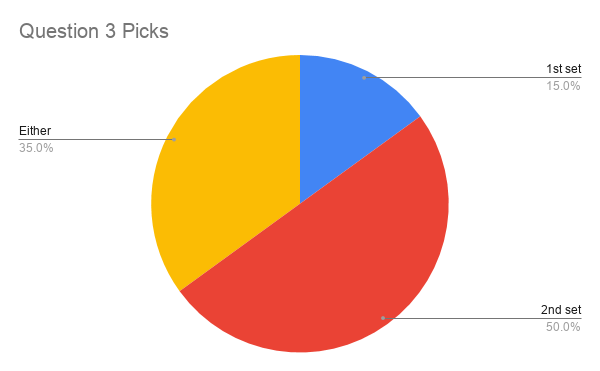
\includegraphics[width=100mm]{Question3Results.png}
                    \caption{Results from Question 3}
                    \label{fig:Question3Results}
                \end{figure}



            \subsubsection{Question 4}

                The fourth question was asked to find out if people thought the system was helpful compared to a normal recommender they may have experienced before. As we can see most users rated it at a four out of five in terms of helpfulness to them. As part of this question, we asked the users to respond with why they found it helpful. We did not pick a recommender that they should compare it too as we are assuming most are familiar with Netflix or a similar movie streaming website even if they are not intimately familiar with how the system works they have has movies recommended to them before. As we can see in figure \ref{fig:Question4Results} the most popular rating was four out of five. Based on feedback provided as well as the results, people found the system helpful but hampered by the fact they had to input movie scores before using the system. and were not greatly fond of having to complete an entire debate to get explanations. This could be just passively given to a user while searching through a streaming service. 

                \begin{figure}
                    \centering
                    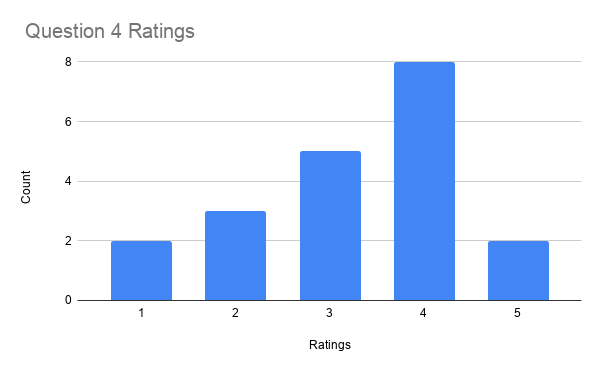
\includegraphics[width=100mm]{Question4Results.png}
                    \caption{Results from Question 4}
                    \label{fig:Question4Results}
                \end{figure}


            \subsubsection{Question 5}
                The fifth question related to whether users found the recommender more interesting to use than a normal recommender. Part of the goal of this recommender was that it would create interesting recommendations. Similar to the last question users felt the system was interesting. Most of the users who tested the system rated it at four out of five \ref{fig:Question5Results}. People found this fun to play with and more interesting that just being shown the movie they might like. 

                \begin{figure}
                    \centering
                    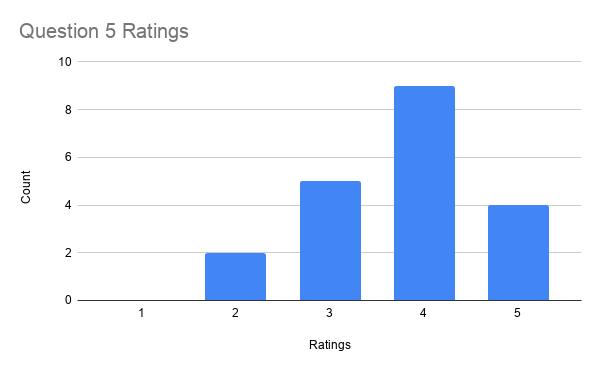
\includegraphics[width=100mm]{Question5Results.png}
                    \caption{Results from Question 5}
                    \label{fig:Question5Results}
                \end{figure}


            \subsubsection{Question 6}
                The last question we asked to find out were any of the explanations particularly interesting to the users. Again this is a subjective question but was mainly to see if users found any particular explanations were helpful while picking a movie. This seemed to vary quite a lot between users as it's up to their tastes. Many liked the information about actors and directors especially if they were aware of who they were. There were also a few votes in favour of genre.
                It would be interesting to implement this into the scoring system based on what movies people removed and increase the weight given to explanations that swung the debate.
        


        \subsection{Conclusions}
            We have seen that most people found the system interesting and it created some explanations that people found helpful and interesting. After completing the user trials we had removed some bugs from the system and gleamed more information about how users feel about the system and how they would use it in practice. This has been very worthwhile and gave us more information about what we can improve about the system in the future. We will explain this in section \ref{sec:FutureWorks}